\section{Preliminary}
\label{sec:pre}

\begin{definition}
\textbf{ Heterogeneous Information Networks (HIN)}\cite{JiSDHG10}. 
Let $T = \{T_1,\ldots, T_m\}$ be a set of $m$ object types.
For each type $T_i$, let $n_i$ and $X_i = {x_i1,\ldots, x_{in_i} }$ be the number and the set of objects of type $Ti$, respectively. An HIN
is a graph $G = (V, E)$, where $V =
\bigcup\limits_{i=1}^{m} X_i$, and $E$ is a set of
links, each represents a binary relation between two objects
in $V$. If $m = 1$ (i.e., there is only one object type), G reduces
to a homogeneous information network. 
\end{definition}

\begin{figure}
    \centering
        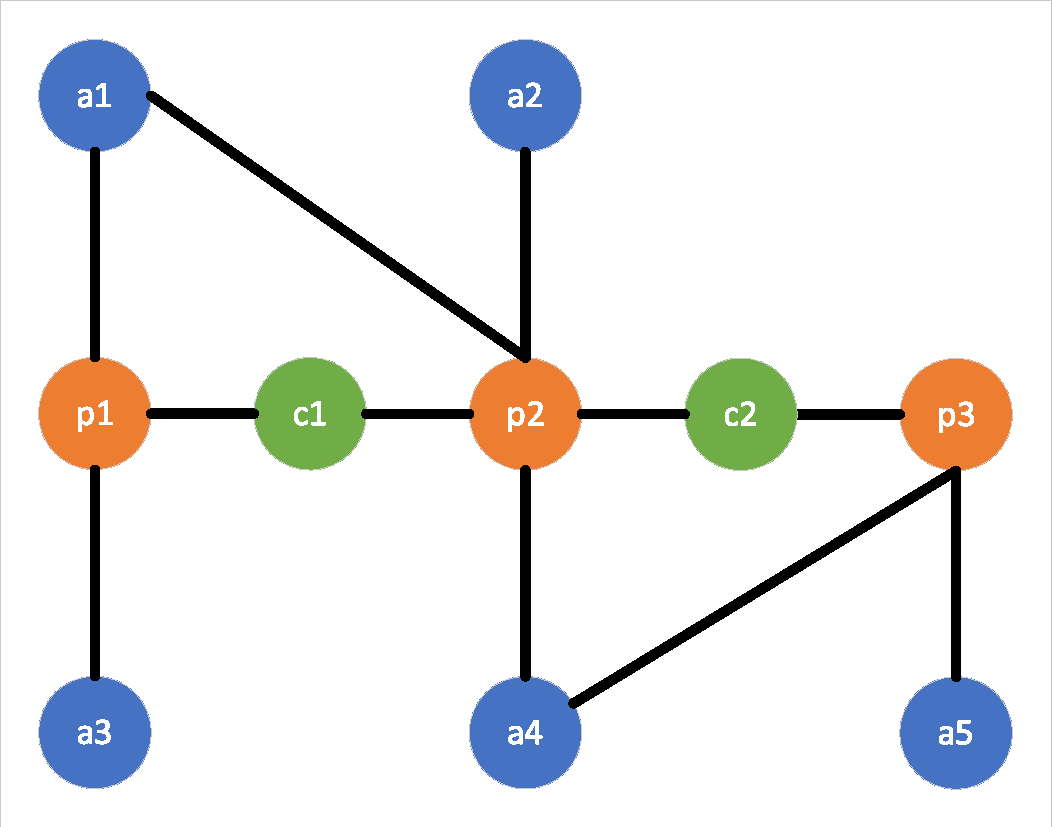
\includegraphics[width = 0.7\linewidth]{figure/example1.pdf}
        \caption{An example of a heterogeneous information network (DBLP). There are three types of nodes (i.e. author, paper, conference).}
        \label{figure:example}
\end{figure}

\begin{example}
In Fig.~\ref{figure:example}, we give an example of HIN. There are three types of nodes, Author, Paper and Conference. And we illustrate two types of edges: Author-Paper, Paper-Conference.
\end{example}

\begin{definition}
\textbf{Metapath}\citep{SunHYYW11}. 
A meta-path $\Phi$ is a path defined on a graph schema. Meta-path $\Phi$: $T_1 \stackrel{R_1}{\longrightarrow} \cdots \stackrel{R_l}{\longrightarrow} T_{l+1}$ defines a composite relation $R = R_1 \circ \cdots \circ R_l$ that relates objects of type $T_1$ to objects of type $T_{l+1}$. 
%If two objects $x_u$ and $x_v$ are related by the composite relation $R$, then there is a path, denoted by $p_{x_u \rightsquigarrow x_v}$, that connects $x_u$ to $x_v$ in $G$. 
We say a path $p = (x_1x_2\ldots x_{l+1})$ between $x_1$ and $x_{l+1}$ in network $G$ follows the meta-path $\Phi$, if each object is of type $T_i$ and each link $ei = \langle x_ix_{i+1}\rangle$ belongs to each relation $R_i$ in $\Phi$. 
We say that $p_{x_1 \rightsquigarrow x_{l+1}}$ is an instance of meta-path $\Phi$, denoted by $p_{x_1 \rightsquigarrow x_{l+1}} \vdash \Phi$.
%We call these paths as path instances of $\Phi$, which are denoted as $p \in \Phi$.
Moreover, in this paper we say $x_v$ is a meta-path $\Phi$ related neighbor of $x_u$, denoted by $x_v \in N^\Phi(x_u)$

\end{definition}

\begin{example}
In Fig.~\ref{figure:example}, $a_3$ is an $APA$-related neighbor of $a_1$, and $a_5$ is an $APCPA$-related neighbor of $a_1$. 
%We have $a_3 \in N^{APA}(a_1)$ and $a_5 \in N^{APCPA}(a_1)$
\end{example}



The notations throughout the rest of paper are shown in Table \ref{table:notation}.


\begin{table}[]
\caption{Description of symbols}
\centering
\begin{tabular}{cc}
\hline
Notation       & Description                                                       \\ \hline
$\Phi$         & Meta-path                                                         \\
$N^\Phi$       & Set of neighbors with respect to a given meta-path $\Phi$          \\
$h^{(t)}$        & Node embedding at layer $t$; $h^{(0)}$ is input node feature \\
$r^{(t)}$        & Edge embedding at layer $t$; $r^{(0)}$ is input edge feature \\
$e_{i,j}^\Phi$ & Similarity of node pair ($i$,$j$) under meta-path $\Phi$   \\
$a_{i,j}^\Phi$ & Attention of node pair ($i$,$j$) under meta-path $\Phi$    \\
$W_F$          & Weight matrix of fully connected layer $F$          \\
$\sigma$       & Sigmoid function                                                  \\
$\oplus$       & Concatenate function \\
$z_i$            & Output embedding for node $i$                                     \\
\hline
\end{tabular}
\label{table:notation}
\end{table}











